\begin{tikzpicture}[
    >=Latex,
    font=\small,
    arr/.style={
        -{Triangle[length=1.2mm,width=1.2mm]},
        line width=0.8pt,
        draw=black
    },
    outarr/.style={
        arr,
        shorten <=1.5pt,
        shorten >=3pt
    },
    sarr/.style={-{Triangle[length=1.2mm,width=1.2mm]}, line width=0.8pt},
    tok/.style={
        draw,
        rounded corners=1pt,
        minimum width=0.24cm,
        minimum height=0.24cm,
        inner sep=0pt,
        line width=0.45pt
    },
    plus/.style={
        circle,
        draw,
        thick,
        inner sep=0pt,
        minimum size=0.32cm,
        font=\scriptsize
    },
    cnode/.style={
        circle,
        draw,
        thick,
        inner sep=0pt,
        minimum size=0.34cm,
        font=\scriptsize
    },
    head/.style={
        draw,
        thick,
        rounded corners=5pt,
        align=center,
        minimum width=0.95cm,
        minimum height=0.55cm,
        inner sep=2pt,
        font=\footnotesize
    },
    imgbox/.style={
        draw,
        thick,
        minimum width=1.25cm,
        minimum height=0.62cm
    }
]

% ------------------------------------------------
% colors
% ------------------------------------------------
\definecolor{pinktok1}{RGB}{246,204,209}
\definecolor{purpletok1}{RGB}{225,210,241}
\definecolor{pinktok2}{RGB}{236,141,152}
\definecolor{purpletok2}{RGB}{189,155,224}
\definecolor{bluetok1}{RGB}{195,225,241}
\definecolor{greentok1}{RGB}{178,221,188}
\definecolor{bluetok2}{RGB}{122,188,224}
\definecolor{greentok2}{RGB}{142,217,115}
\definecolor{yellowtok}{RGB}{246,212,120}
\definecolor{cyantok}{RGB}{190,226,226}

\colorlet{layerbg}{white}

\newcommand{\gradtok}[4]{
\shade[
    draw=black,
    rounded corners=1pt,
    line width=0.45pt,
    left color=#3,
    right color=#4,
]
    ($(#1,#2)+(-0.12,-0.12)$)
    rectangle
    ($(#1,#2)+(0.12,0.12)$);
}

% ------------------------------------------------
% helper commands
% ------------------------------------------------
\newcommand{\imagestack}[2]{
\begin{scope}[shift={(#1,#2)}]
    \draw[fill=gray!15, draw=gray!45] (-0.68,-0.22) rectangle (0.68,0.54);
    \draw[fill=gray!10, draw=gray!45] (-0.58,-0.30) rectangle (0.78,0.46);
    \draw[fill=gray!5,  draw=gray!45] (-0.48,-0.38) rectangle (0.88,0.38);
\end{scope}
}

\newcommand{\imagestacks}[3]{
\begin{scope}[shift={(#1,#2)}]
    \node[inner sep=0pt] at (0,0.32) {
        \includegraphics[width=1.36cm,height=0.76cm]{assets/#3_1}
    };
    \node[inner sep=0pt] at (0.20,0.16) {
        \includegraphics[width=1.36cm,height=0.76cm]{assets/#3_2}
    };
    \node[inner sep=0pt] at (0.40,0.00) {
        \includegraphics[width=1.36cm,height=0.76cm]{assets/#3_3}
    };
\end{scope}
}

\newcommand{\cameras}[2]{
\begin{scope}[shift={(#1,#2)}]
    \foreach \i in {0,...,2}{
        \node[inner sep=0pt] at (0.135,{0.10-0.42*\i}) {
            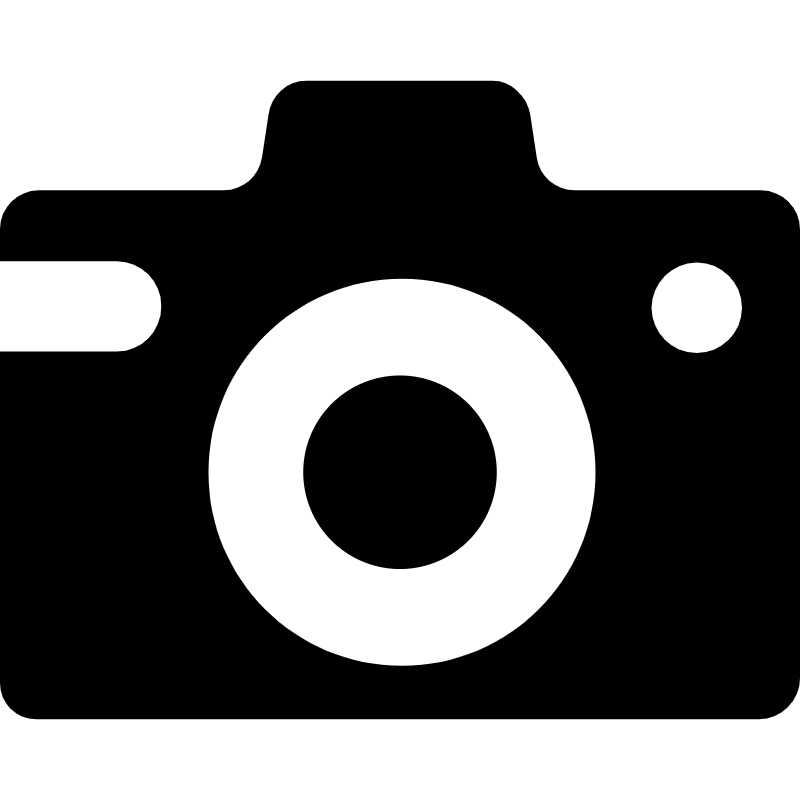
\includegraphics[width=0.27cm]{assets/camera2.png}
        };
    }
\end{scope}
}

\newcommand{\pairblock}[6]{
\begin{scope}[shift={(#1,#2)}]
    \draw[dotted, thick, rounded corners=4pt] (-0.50,0.58) rectangle (0.88,-1.96);
    \node[font=\scriptsize] at (-0.25,0.36) {$#5$};
    \node[font=\scriptsize] at (0.62,0.36) {$#6$};

    \foreach \i in {0,...,5}{
        \node[tok, fill=#3] at (-0.25,{-0.10-0.30*\i}) {};
        \node[tok, fill=#4] at (0.62,{-0.10-0.30*\i}) {};
    }

    \node[plus] at (0.18,-0.83) {$+$};
\end{scope}
}

\newcommand{\ctokens}[4]{
\begin{scope}[shift={(#1,#2)}]
    \node[tok, fill=yellowtok] at (-0.22,0.83) {};
    \node[tok, fill=yellowtok] at (0.22,0.83) {};
    \node[font=\scriptsize] at (-0.22,1.25) {$#3$};
    \node[font=\scriptsize] at (0.22,1.25) {$#4$};

    \draw[sarr] (0,0.65) -- (0,0.22);
    \node[cnode] at (0,0) {\textbf{c}};
\end{scope}
}

\newcommand{\fblock}[8]{
\begin{scope}[shift={(#1,#2)}]
    \node[font=\scriptsize] at (-0.23,0.42) {$#7$};
    \node[font=\scriptsize] at (0.32,0.42) {$#8$};

    \node[tok, fill=yellowtok] at (-0.23,0) {};
    \node[tok, fill=yellowtok] at (0.32,0) {};
    \foreach \i in {1,...,6}{
        \gradtok{-0.23}{-0.30*\i}{#3}{#4}
        \gradtok{0.32}{-0.30*\i}{#5}{#6}
    }
\end{scope}
}

\newcommand{\patchtokens}[2]{
\begin{scope}[shift={(#1,#2)}]
    \node at (0.22,0.62) {patch token};

    \gradtok{0.00}{0.18}{pinktok1}{purpletok1}
    \gradtok{0.14}{0.10}{pinktok2}{purpletok2}
    \gradtok{0.28}{0.02}{bluetok1}{greentok1}
    \gradtok{0.42}{-0.06}{bluetok2}{greentok2}
\end{scope}
}

\newcommand{\cameratokens}[2]{
\begin{scope}[shift={(#1,#2)}]
    \foreach \i in {0,...,3}{
        \node[tok, fill=yellowtok] at ({0.14*\i},{-0.08*\i}) {};
    }
    \node at (0.45,-0.58) {camera token};
\end{scope}
}

\newcommand{\outputimg}[3]{
\begin{scope}[shift={(#1,#2)}]
    \node[
        inner sep=0pt,
        draw=black,
        line width=0.35pt,
        opacity=0.65
    ] at (0,0.18) {
        \includegraphics[width=1.25cm,height=0.62cm]{#3_1}
    };
    \node[
        inner sep=0pt,
        draw=black,
        line width=0.35pt,
        opacity=0.85
    ] at (0.18,0.09) {
        \includegraphics[width=1.25cm,height=0.62cm]{#3_2}
    };
    \node[
        inner sep=0pt,
        draw=black,
        line width=0.35pt,
        opacity=1
    ] at (0.36,0.00) {
        \includegraphics[width=1.25cm,height=0.62cm]{#3_3}
    };
\end{scope}
}

% ------------------------------------------------
% left input part
% ------------------------------------------------
\node[font=\bfseries\normalsize] at (0.95,5.35) {Input Data};

\draw[->, thick] (0.35,0.85) -- (0.35,5.02);
\node at (-0.02,2.90) {$V$};

\draw[->, thick] (0.35,0.85) -- (0.98,0.25);
\node at (0.48,0.25) {$T$};

\imagestacks{1.25}{4.25}{input1}
\imagestacks{1.25}{1.08}{input2}

\foreach \y in {3.25,2.85,2.45}{
    \fill (1.55,\y) circle (1.15pt);
}

\cameras{2.55}{4.70}
\cameras{2.55}{1.63}

\draw[arr] (2.95,4.12) -- (3.65,4.12);
\draw[arr] (2.95,1.05) -- (3.65,1.05);

% ------------------------------------------------
% token construction
% ------------------------------------------------
\pairblock{4.20}{4.95}{pinktok1}{purpletok1}{X_{1}^{v}}{R_{1}^{v}}
\pairblock{5.85}{4.95}{pinktok2}{purpletok2}{X_{t}^{v}}{R_{t}^{v}}

\draw[arr] (6.78,4.12) -- (7.16,4.12);

\ctokens{7.415}{4.12}{C_{1}^{v}}{C_{t}^{v}}

\draw[arr] (7.67,4.12) -- (8.05,4.12);

\fblock{8.45}{4.95}{pinktok1}{purpletok1}{pinktok2}{purpletok2}{Z_{1}^{v}}{Z_{t}^{v}}

\pairblock{4.20}{1.88}{bluetok1}{greentok1}{X_{1}^{1}}{R_{1}^{1}}
\pairblock{5.85}{1.88}{bluetok2}{greentok2}{X_{t}^{1}}{R_{t}^{1}}

\draw[arr] (6.78,1.05) -- (7.16,1.05);

\ctokens{7.415}{1.05}{C_{1}^{v}}{C_{t}^{v}}

\draw[arr] (7.67,1.05) -- (8.05,1.05);

\fblock{8.45}{1.88}{bluetok1}{greentok1}{bluetok2}{greentok2}{Z_{1}^{1}}{Z_{t}^{1}}

\draw[arr] (8.95,4.12) -- (9.85,4.12);
\draw[arr] (8.95,1.05) -- (9.85,1.05);

% ------------------------------------------------
% attention layers
% ------------------------------------------------
\node[fill=layerbg, inner sep=1pt] at (11.18,5.10) {$\times\ L$ Layers};

\filldraw[draw=black, fill=layerbg, thick, rounded corners=11pt]
    (10.35,0.85) rectangle (12.75,4.85);

\filldraw[draw=black, fill=layerbg, thick, rounded corners=11pt]
    (10.15,0.70) rectangle (12.55,4.70);

\filldraw[draw=black, fill=layerbg, thick, rounded corners=11pt]
    (9.95,0.55) rectangle (12.35,4.55);

% attention module horizontal adjustment
\def\AttnXShift{-0.05}

\node[
    draw, fill=layerbg, thick, rounded corners=5pt,
    minimum width=0.42cm, minimum height=3.05cm
] at ({10.5+\AttnXShift},2.55) {};

\node[
    draw, fill=layerbg, thick, rounded corners=5pt,
    minimum width=0.42cm, minimum height=3.05cm
] at ({11.2+\AttnXShift},2.55) {};

\node[
    draw, fill=layerbg, thick, rounded corners=5pt,
    minimum width=0.42cm, minimum height=3.05cm
] at ({11.9+\AttnXShift},2.55) {};

\node[rotate=270, font=\footnotesize, fill=layerbg, inner sep=1pt] at ({10.5+\AttnXShift},2.55) {Self Attention};
\node[rotate=270, font=\footnotesize, fill=layerbg, inner sep=1pt] at ({11.2+\AttnXShift},2.55) {Temporal Attention};
\node[rotate=270, font=\footnotesize, fill=layerbg, inner sep=1pt] at ({11.9+\AttnXShift},2.55) {View Attention};

% ------------------------------------------------
% output tokens
% ------------------------------------------------
\draw[thick] (12.75,2.30) -- (13.10,2.30);
\draw[thick] (13.10,2.30) -- (13.10,3.75);
\draw[thick] (13.10,2.30) -- (13.10,1.05);

\draw[thick] (13.10,3.75) -- (13.55,3.75);
\draw[thick] (13.10,1.05) -- (13.55,1.05);

\patchtokens{13.75}{3.66}
\cameratokens{13.72}{1.15}

% ------------------------------------------------
% heads and routes
% ------------------------------------------------
\draw[thick] (14.42,3.75) -- (15.10,3.75);
\draw[thick] (15.10,3.75) -- (15.10,4.95);
\draw[thick] (15.10,3.75) -- (15.10,2.55);

\draw[arr] (15.10,4.95) -- (15.55,4.95);
\draw[arr] (15.10,3.75) -- (15.55,3.75);
\draw[arr] (15.10,2.55) -- (15.55,2.55);

\draw[arr] (14.35,1.05) -- (15.35,1.05);

\node[head] (dpt) at (16.05,4.95) {Depth\\Head};
\node[head] (occ) at (16.05,3.75) {Occ\\Head};
\node[head] (det) at (16.05,2.55) {Det\\Head};
\node[head] (cam) at (16.05,1.05) {Camera\\Head};


% ------------------------------------------------
% output image boxes
% The output arrows use outarr to keep gaps from both heads and outputs.
% ------------------------------------------------
\draw[outarr] (dpt.east) -- (17.20,4.95);
\outputimg{17.8}{4.95}{assets/dpt_out};

\draw[outarr] (occ.east) -- (17.20,3.75);
\outputimg{17.8}{3.75}{assets/occ_out};

\draw[outarr] (det.east) -- (17.20,2.55);
\outputimg{17.8}{2.55}{assets/det_out};

\draw[outarr] (cam.east) -- (17.20,1.05);
\node[
inner sep=0pt,
draw=black,
line width=0.05pt
] at (18,1.05) {
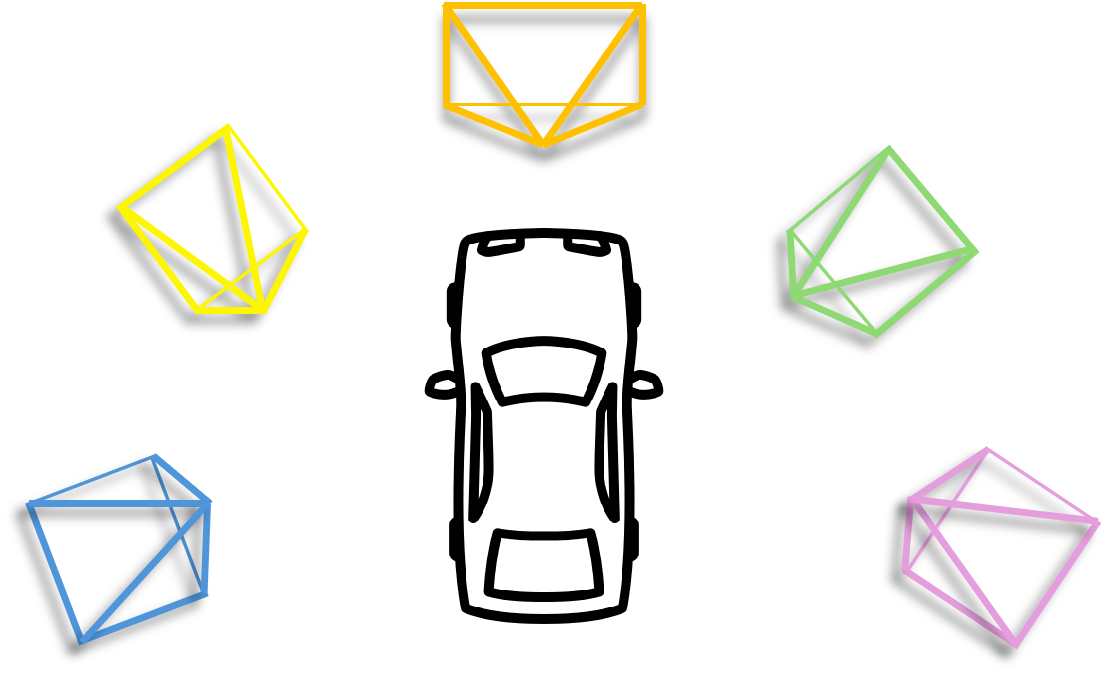
\includegraphics[width=1.5cm,height=1cm]{assets/camera_out.png}
};



\end{tikzpicture}
